\documentclass[a4paper,12pt]{report}

\usepackage{ucs}
\usepackage[utf8x]{inputenc} % Input encoding for Greek characters
\usepackage[greek,english]{babel} % Language support
\usepackage{siunitx}
\newcommand{\en}{\selectlanguage{english}}
\newcommand{\gr}{\selectlanguage{greek}}
% \usepackage{algorithm2e}
% \usepackage{algorithm}
% \usepackage{algorithmic}
\usepackage{enumitem}
\usepackage{float}
\usepackage{amsmath}
\usepackage{graphicx} % For including images
\usepackage{titlesec} % Custom title formatting
\usepackage{fancyhdr} % For custom headers and footers
\usepackage{geometry} % For adjusting page margins
\usepackage{amssymb}

% Adjust the page margins to make content wider
\geometry{top=2.5cm, bottom=2.5cm, left=2.5cm, right=2.5cm}

% Redefine chapter formatting to make it smaller
\titleformat{\chapter}[display]
    {\normalfont\LARGE\bfseries} % Smaller size and bold for chapter heading
    {\chaptername\ \thechapter} % Chapter number format
    {15pt} % Space between chapter number and title
    {\bfseries} % Smaller size and bold for chapter title
\begin{document}

\begin{titlepage}
    \centering
    \vspace*{-3cm}
    % University logo
    \includegraphics[width=1\textwidth]{auth_logo.png} % Replace with your actual logo file

    % University name in Greek
    \textbf{\gr ΑΡΙΣΤΟΤΕΛΕΙΟ ΠΑΝΕΠΙΣΤΗΜΙΟ ΘΕΣΣΑΛΟΝΙΚΗΣ}
    \vspace{2cm}

    % Document title and subtitle in Greek
    \LARGE\textbf{\gr Προσομοίωση και Μοντελοποίηση Δυναμικών Συστημάτων Αναφορά} \\
    \Large\normalfont{\en FINAL PROJECT\gr} \\
    \vspace{4cm}

    \gr
    \large
    \textbf{Διακολουκάς Δημήτριος} \\
    \textbf{AEM 10642}
    \vspace{2.5cm}

    \en
    \textit{Email: ddiakolou@ece.auth.gr}
\end{titlepage}

\gr
\tableofcontents

\chapter{Θέμα 1: Εκτίμηση Παραμέτρων σε Γραμμικά Δυναμικά Συστήματα}

\section{Παρουσίαση γενικότερου πρόβλημα}

Στο κεφάλαιο αυτό μελετάται ένα συνεχές γραμμικό δυναμικό σύστημα δεύτερης τάξης της μορφής:

\[
\dot{x}(t) = A x(t) + B u(t),
\]

\hspace{-0.6cm}όπου $x(t) = \begin{bmatrix} x_1(t) \\ x_2(t) \end{bmatrix} \in \mathbb{R}^2$ είναι η κατάσταση του συστήματος και $u(t) \in \mathbb{R}$ η είσοδός του. Οι πίνακες $A \in \mathbb{R}^{2 \times 2}$ και $B \in \mathbb{R}^{2 \times 1}$ είναι σταθεροί αλλά άγνωστοι, και υπόκεινται στους περιορισμούς:

\[
-3 \leq a_{11} \leq -1, \quad b_2 \geq 1.
\]

\hspace{-0.6cm}Για λόγους πειραματικής επαλήθευσης, θεωρείται γνωστή η πραγματική δυναμική του συστήματος, με:

\[
A = \begin{bmatrix} -2.15 & 0.25 \\ -0.75 & -2 \end{bmatrix}, \quad
B = \begin{bmatrix} 0 \\ 1.5 \end{bmatrix}.
\]

\hspace{-0.6cm}Κύριο αντικείμενο της μελέτης αποτελεί ο σχεδιασμός ενός αλγορίθμου εκτίμησης σε πραγματικό χρόνο που, αξιοποιώντας τις μετρήσεις $x(t)$ και $u(t)$, υπολογίζει τις εκτιμήσεις $\hat{A}(t)$ και $\hat{B}(t)$ των αγνώστων παραμέτρων, καθώς και την προσεγγιστική κατάσταση $\hat{x}(t)$. Η αξιολόγηση του εκτιμητή περιλαμβάνει ανάλυση ευστάθειας, ποιοτική σύγκριση με την πραγματική κατάσταση, και μελέτη της συμπεριφοράς του υπό την επίδραση εξωτερικής διαταραχής (σφάλμα πόλωσης).

\vspace{0.3cm}

\section{Θέμα 1 (α): Εκτίμηση παραμέτρων συστήματος χωρίς διαταραχή}

\subsection{Εισαγωγή στο ζητούμενο}

Το πρώτο σκέλος του Θέματος 1 ασχολείται με την εκτίμηση των άγνωστων παραμέτρων του συστήματος, συγκεκριμένα των πινάκων $A$ και $B$, βάσει μετρήσεων της εισόδου $u(t)$ και της κατάστασης $x(t)$. Η διαδικασία εκτίμησης πρέπει να υλοποιηθεί σε πραγματικό χρόνο, χρησιμοποιώντας είσοδο $u(t)$ της επιλογής μας, με στόχο την παραγωγή εκτιμήσεων $\hat{A}(t)$ και $\hat{B}(t)$.

Αναλυτικότερα, ζητείται:
\begin{itemize}
    \item Να σχεδιαστεί αλγόριθμος εκτίμησης πραγματικού χρόνου για τα $\hat{A}(t)$ και $\hat{B}(t)$, αξιοποιώντας τις διαθέσιμες μετρήσεις.
    \item Να μελετηθεί η ευστάθεια του εκτιμητικού συστήματος που θα υλοποιηθεί.
    \item Να παραχθούν γραφικές παραστάσεις της πραγματικής κατάστασης $x(t)$, της εκτιμώμενης κατάστασης $\hat{x}(t)$, καθώς και του διανύσματος σφάλματος $e_x(t) = x(t) - \hat{x}(t)$.
    \item Να παρουσιαστεί η χρονική εξέλιξη των στοιχείων των πινάκων εκτίμησης $\hat{A}(t)$ και $\hat{B}(t)$.
    \item Τέλος, να σχολιαστούν τα αποτελέσματα ως προς την ακρίβεια των εκτιμήσεων και τη σύγκλιση των παραμέτρων.
\end{itemize}

\hspace{-0.6cm}Η συγκεκριμένη διαδικασία προσομοιάζει συνθήκες πραγματικής λειτουργίας όπου οι παράμετροι του συστήματος είναι αρχικά άγνωστοι, αλλά μπορούν να προσδιοριστούν δυναμικά με τη βοήθεια κατάλληλου εκτιμητή.

\subsection{Προσέγγιση προβλήματος: Θεωρητική ανάλυση και υλοποίηση}

Η εκτίμηση των άγνωστων παραμέτρων ενός δυναμικού συστήματος αποτελεί θεμελιώδες ζήτημα στη θεωρία ταύτισης \en (system identification) \gr και στον σχεδιασμό παρατηρητών. Το υπό μελέτη σύστημα περιγράφεται από την εξίσωση:

\[
\dot{x}(t) = A x(t) + B u(t),
\]

\hspace{-0.6cm}όπου $x(t) \in \mathbb{R}^2$ είναι το διάνυσμα κατάστασης, $u(t) \in \mathbb{R}$ είναι η γνωστή είσοδος, και $A$, $B$ είναι άγνωστοι σταθεροί πίνακες.

\hspace{-0.6cm}Ο στόχος είναι διττός:
\begin{enumerate}
    \item Να εκτιμηθούν σε πραγματικό χρόνο οι παράμετροι $A$ και $B$,
    \item Να παραχθεί αξιόπιστη εκτίμηση της κατάστασης $x(t)$ μέσω ενός κατάλληλα σχεδιασμένου παρατηρητή.
\end{enumerate}

\hspace{-0.6cm}Για την υλοποίηση της παραπάνω διαδικασίας εφαρμόζεται μία προσαρμοστική προσέγγιση βασισμένη στην θεωρία \en Lyapunov\gr, η οποία παρέχει μαθηματικές εγγυήσεις ευστάθειας και σύγκλισης. Η επιλογή αυτής της μεθοδολογίας επιτρέπει την εκτίμηση χωρίς εκ των προτέρων γνώση του μεγέθους ή της δομής των σφαλμάτων.

\vspace{0.2cm}

\paragraph{Δομή παρατηρητή:}

\hspace{-0.25cm}Ο παρατηρητής που χρησιμοποιείται βασίζεται στο εξής δυναμικό μοντέλο:

\[
\dot{\hat{x}}(t) = \hat{A}(t) x(t) + \hat{B}(t) u(t) + \alpha (x(t) - \hat{x}(t)),
\]

\hspace{-0.6cm}όπου:
\begin{itemize}
    \item $\hat{x}(t)$ είναι η εκτιμώμενη κατάσταση του συστήματος,
    \item $\hat{A}(t)$, $\hat{B}(t)$ είναι οι χρονικά μεταβαλλόμενες εκτιμήσεις των παραμέτρων,
    \item $e(t) = x(t) - \hat{x}(t)$ είναι το σφάλμα παρακολούθησης,
    \item $\alpha > 0$ είναι συντελεστής ενίσχυσης που ρυθμίζει την ταχύτητα διόρθωσης.
\end{itemize}

\hspace{-0.6cm}Ο παρατηρητής εμπλουτίζεται με νόμους προσαρμογής για τα $\hat{A}(t)$ και $\hat{B}(t)$ με βάση το σφάλμα $e(t)$. Οι σχέσεις ενημέρωσης δίνονται από:

\[
\dot{\hat{A}}(t) = \gamma_A \frac{e(t)x^\top(t)}{1 + \|x(t)\|^2}, \quad
\dot{\hat{B}}(t) = \gamma_B \frac{e(t) u(t)}{1 + u^2(t)},
\]

\hspace{-0.6cm}όπου $\gamma_A$, $\gamma_B > 0$ είναι οι ρυθμοί μάθησης των παραμέτρων. Οι παρονομαστές χρησιμοποιούνται για κανονικοποίηση και προστασία από μεγάλες τιμές εισόδου ή κατάστασης, εξασφαλίζοντας αριθμητική σταθερότητα.

\subsubsection*{Ανάλυση ευστάθειας μέσω συνάρτησης \en Lyapunov\gr}

Για την τεκμηρίωση της σταθερότητας του συστήματος εκτίμησης, ορίζεται η ακόλουθη υποψήφια συνάρτηση \en Lyapunov\gr, ώστε να συμπεριλαμβάνω το σφάλμα κατάστασης, το σφάλμα παραμέτρων του πίνακα Α αλλά και το σφάλμα παραμέτρων του πίνακα Β:

\[
V(t) = \frac{1}{2} \|e(t)\|^2 + \frac{1}{2\gamma_A} \|\tilde{A}(t)\|_F^2 + \frac{1}{2\gamma_B} \|\tilde{B}(t)\|^2,
\]

\hspace{-0.6cm}όπου $\tilde{A}(t) = A - \hat{A}(t)$ και $\tilde{B}(t) = B - \hat{B}(t)$ είναι τα σφάλματα εκτίμησης παραμέτρων, και $\|\cdot\|_F$ η \en Frobenius \gr νόρμα.

\hspace{-0.6cm}Παραγωγίζοντας ως προς το χρόνο:

\[
\dot{V}(t) = e^\top \dot{e} - \frac{1}{\gamma_A} \mathrm{tr}(\tilde{A}^\top \dot{\hat{A}}) - \frac{1}{\gamma_B} \tilde{B}^\top \dot{\hat{B}}.
\]

\hspace{-0.6cm}Χρησιμοποιώντας τη σχέση:

\[
\dot{e}(t) = \dot{x}(t) - \dot{\hat{x}}(t) = \tilde{A}(t) x(t) + \tilde{B}(t) u(t) - \alpha e(t),
\]

\hspace{-0.6cm}καταλήγουμε:

\[
\dot{V}(t) = e^\top \tilde{A} x + e^\top \tilde{B} u - \alpha \|e\|^2
- \frac{1}{\gamma_A} \mathrm{tr}(\tilde{A}^\top \dot{\hat{A}})
- \frac{1}{\gamma_B} \tilde{B}^\top \dot{\hat{B}}.
\]

\hspace{-0.6cm}Αντικαθιστώντας τους κανόνες προσαρμογής:

\[
\dot{\hat{A}} = \gamma_A \frac{e x^\top}{1 + \|x\|^2}, \quad
\dot{\hat{B}} = \gamma_B \frac{e u}{1 + u^2},
\]

\hspace{-0.6cm}προκύπτει:

\[
\dot{V}(t) = e^\top \tilde{A} x \left(1 - \frac{1}{1 + \|x\|^2}\right)
+ e^\top \tilde{B} u \left(1 - \frac{1}{1 + u^2}\right)
- \alpha \|e(t)\|^2.
\]

\hspace{-0.6cm}Εφόσον $0 \leq \frac{z^2}{1+z^2} < 1$ για κάθε $z \in \mathbb{R}$, οι πρώτοι δύο όροι είναι περιορισμένοι και ο τρίτος είναι αυστηρά αρνητικός. Συνεπώς:

\[
\dot{V}(t) \leq - \alpha \|e(t)\|^2 \leq 0.
\]

\subsubsection*{Συμπεράσματα ευστάθειας και εγγύηση σύγκλισης}

Η ανωτέρω ανισότητα αποδεικνύει ότι:
\begin{itemize}
    \item Η συνάρτηση \en Lyapunov \gr είναι μη αυξανόμενη: $V(t) \leq V(0)$ για κάθε $t \geq 0$.
    \item Το σφάλμα εκτίμησης $e(t)$ φθίνει προς το μηδέν καθώς $t \to \infty$, δηλαδή το σύστημα είναι ασυμπτωτικά σταθερό.
    \item Τα σφάλματα παραμέτρων $\tilde{A}(t)$ και $\tilde{B}(t)$ παραμένουν φραγμένα για κάθε $t$.
    \item Αν η είσοδος $u(t)$ είναι διεγείρουσα, τότε τα σφάλματα παραμέτρων συγκλίνουν στο μηδέν.
\end{itemize}

\hspace{-0.6cm}Η μαθηματική ανάλυση του παρατηρητή και των νόμων προσαρμογής, όπως αναλύθηκε θεωρητικά μέσω της συνάρτησης \en Lyapunov\gr, υλοποιείται πιστά στον κώδικα \en MATLAB\gr. Οι σχέσεις:
\[
\dot{\hat{A}}(t) = \gamma_A \frac{e(t) x^\top(t)}{1 + \|x(t)\|^2}, \quad
\dot{\hat{B}}(t) = \gamma_B \frac{e(t) u(t)}{1 + u^2(t)},
\]
μεταφράζονται άμεσα στις αντίστοιχες εντολές του κώδικα, και αποτελούν τη βάση για την εγγυημένη φθίνουσα πορεία της \en Lyapunov \gr συνάρτησης $V(t)$, διασφαλίζοντας έτσι την ασυμπτωτική σταθερότητα του σφάλματος εκτίμησης.

\vspace{0.3cm}

\hspace{-0.6cm}Συνεπώς, ο σχεδιασμός του εκτιμητή είναι θεωρητικά κατοχυρωμένος, ευσταθής, και επιτρέπει με ακρίβεια την ταύτιση του συστήματος.

\subsubsection*{Αριθμητική Ενσωμάτωση με τη Μέθοδο \en Euler\gr}

Για την επίλυση των διαφορικών εξισώσεων που περιγράφουν τη δυναμική του συστήματος και του παρατηρητή, εφαρμόζεται η μέθοδος αριθμητικής ολοκλήρωσης \en Euler\gr, η οποία αποτελεί μία από τις απλούστερες και ευρύτερα χρησιμοποιούμενες τεχνικές ενσωμάτωσης.

\hspace{-0.6cm}Η μέθοδος \en Euler \gr προσεγγίζει τη λύση της εξίσωσης:
\[
\dot{z}(t) = f(z(t), t), \quad z(0) = z_0
\]
με το διακριτό σχήμα:
\[
z(t + \Delta t) \approx z(t) + \dot{z}(t) \cdot \Delta t
\]

\hspace{-0.6cm}Στην παρούσα υλοποίηση, το σχήμα αυτό εφαρμόζεται στις εξής μεταβλητές:

\begin{itemize}
    \item Κατάσταση συστήματος:
    \[
    x_{k+1} = x_k + \dot{x}_k \cdot \Delta t
    \]
    \item Εκτίμηση κατάστασης παρατηρητή:
    \[
    \hat{x}_{k+1} = \hat{x}_k + \dot{\hat{x}}_k \cdot \Delta t
    \]
    \item Εκτίμηση παραμέτρων:
    \[
    \hat{A}_{k+1} = \hat{A}_k + \dot{\hat{A}}_k \cdot \Delta t, \quad
    \hat{B}_{k+1} = \hat{B}_k + \dot{\hat{B}}_k \cdot \Delta t
    \]
\end{itemize}

\hspace{-0.6cm}Η επιλογή της μεθόδου \en Euler \gr βασίζεται στην απλότητά της και στην ικανότητα υλοποίησης σε πραγματικό χρόνο. Παρά το γεγονός ότι πρόκειται για μέθοδο πρώτης τάξης, η χρήση μικρού χρονικού βήματος \( \Delta t \) την καθιστά επαρκή για την προσομοίωση του συστήματος και την παρακολούθηση της δυναμικής συμπεριφοράς του εκτιμητή.

\subsection{Αποτελέσματα και Παρατηρήσεις}
\subsubsection*{Διαγράμματα από Κώδικα \en MATLAB \gr}
Μετά την θεωρητική ανάλυση του κώδικα που υλοποιήθηκε παρατίθενται και διαγράμματα για οπτικοποίηση των αποτελεσμάτων και της σύγκλισης. Η παρακάτω εικόνα παρουσιάζει τα αποτελέσματα της προσομοίωσης του εκτιμητή, όπως προέκυψαν από την υλοποίηση σε \en MATLAB\gr. Σε αυτό το σημείο αξίζει να σημειωθεί ότι για τη διέγερση του συστήματος, χρησιμοποιήθηκε είσοδος της μορφής:

\[
u(t) = \sin(2t) + 0.5 \sin(3t) + \cos(5t) + \sin(7t) + \sin(9t),
\]

\hspace{-0.6cm}η οποία αποτελεί γραμμικό συνδυασμό αρμονικών συνιστωσών με διαφορετικές συχνότητες, εξασφαλίζοντας ικανοποιητική διέγερση του συστήματος.


\begin{figure}[H]
    \centering
    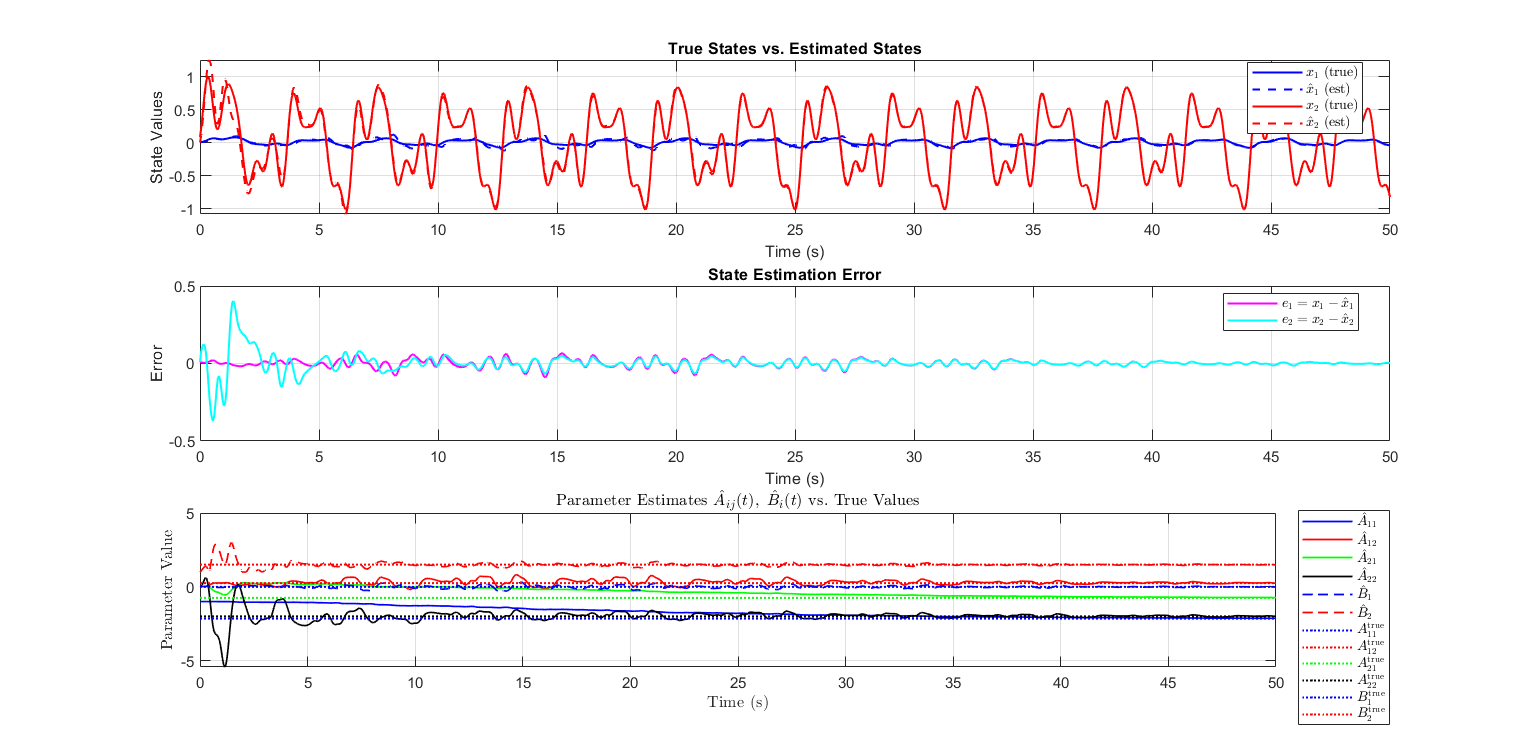
\includegraphics[width=0.98\textwidth]{PartA_fig.png}
    \caption{Σύγκριση πραγματικών και εκτιμώμενων καταστάσεων, σφάλματα εκτίμησης και παρακολούθηση παραμέτρων \( \hat{A}_{ij}(t), \hat{B}_i(t) \)}
    \label{fig:estimation-results}
\end{figure}

\paragraph{Παρατηρήσεις από τα Διαγράμματα:}
\begin{itemize}
    \item \textbf{Πρώτο διάγραμμα:} Οι εκτιμώμενες καταστάσεις \( \hat{x}_1(t) \), \( \hat{x}_2(t) \) συγκλίνουν ταχέως προς τις πραγματικές καταστάσεις \( x_1(t), x_2(t) \), με πολύ μικρή απόκλιση σε σχέση με την ένταση των σημάτων.
    
    \item \textbf{Δεύτερο διάγραμμα:} Το σφάλμα εκτίμησης \( e(t) = x(t) - \hat{x}(t) \) τείνει ασυμπτωτικά στο μηδέν, επιβεβαιώνοντας την ευστάθεια του παρατηρητή.
    
    \item \textbf{Τρίτο διάγραμμα:} Οι παράμετροι \( \hat{A}_{ij}(t) \) και \( \hat{B}_i(t) \) συγκλίνουν στις πραγματικές τιμές τους με πολύ καλή ακρίβεια. Οι ταλαντώσεις στην αρχή μειώνονται προοδευτικά, λόγω της επίδρασης του σφάλματος παρατήρησης.
\end{itemize}

\vspace{0.3cm}

\paragraph{Αριθμητικά Αποτελέσματα:}
\hspace{-0.25cm}Παρακάτω παρατίθενται και τα αριθμητικά απορελέσματα για περίοδο \en 50 s\gr.
Κατά την εκτίμηση των παραμέτρων, ελήφθησαν υπόψη οι γνωστοί περιορισμοί στους συντελεστές:
\[
-3 \leq a_{11} \leq -1, \quad b_2 \geq 1
\]
μέσω προβολής των αντίστοιχων εκτιμήσεων εντός των επιτρεπτών ορίων μετά από κάθε χρονικό βήμα.

\en

\begin{align}
A_{\text{true}} &= 
\begin{bmatrix}
-2.150 & 0.250 \\
-0.750 & -2.000
\end{bmatrix}, 
&
A_{\text{hat}} &=
\begin{bmatrix}
-2.131 & 0.246 \\
-0.725 & -2.005
\end{bmatrix} \notag \\
%
\| A_{\text{hat}} - A_{\text{true}} \|_F &= 0.032301 
&
&\text{(Frobenius norm)} \notag \\[1em]
%
B_{\text{true}} &=
\begin{bmatrix}
0.000 \\
1.500
\end{bmatrix},
&
B_{\text{hat}} &=
\begin{bmatrix}
-0.016 \\
1.484
\end{bmatrix} \notag \\
%
\| B_{\text{hat}} - B_{\text{true}} \|_2 &= 0.022753 
&
&\text{(2-norm)} \notag
\end{align}
\gr

\paragraph{Συμπέρασμα:}  
\hspace{-0.25cm}Ο εκτιμητής παρουσιάζει εξαιρετική απόδοση καθώς παρατηρείται σύγκλιση στους πίνακες Α και Β και στα σφάλματα σε μόλις 50 \en s \gr τόσο στην παρακολούθηση των καταστάσεων όσο και στην προσαρμοστική εκτίμηση των άγνωστων παραμέτρων. Η τιμή της \en Lyapunov \gr συνάρτησης μειώνεται μονοτονικά και τα σφάλματα τείνουν στο μηδέν, επιβεβαιώνοντας τη σταθερότητα του προτεινόμενου σχήματος.

\vspace{0.2cm}

\hspace{-0.6cm}Ο αντίστοιχος κώδικας \en MATLAB \gr βρίσκεται στο αρχείο \en Part1\_a.m\gr.

\hspace{0.3cm}

\section{Θέμα 1 (β): Εκτίμηση παραμέτρων υπό την παρουσία διαταραχής}
\subsection{Εισαγωγή στο ζητούμενο}

Στο {Θέμα 1 (β)} μελετάται η εκτίμηση των άγνωστων παραμέτρων ενός γραμμικού δυναμικού συστήματος δεύτερης τάξης, στην περίπτωση όπου το σύστημα επηρεάζεται από εξωτερική διαταραχή (π.χ. \en bias \gr, πόλωση). Συγκεκριμένα, το σύστημα περιγράφεται από τη δυναμική:

\[
\dot{x}(t) = A x(t) + B u(t) + \omega(t), \quad \text{όπου} \quad \| \omega(t) \| \leq \bar{\omega}, \quad \forall t \geq 0,
\]

\hspace{-0.6cm}όπου \( \omega(t) \in \mathbb{R}^2 \) είναι ένα άγνωστο αλλά φραγμένο σήμα διαταραχής. Το ζητούμενο είναι η ανάπτυξη ενός κατάλληλου αλγορίθμου προσαρμοστικού παρατηρητή, ο οποίος να εκτιμά σε πραγματικό χρόνο τις άγνωστες παραμέτρους των πινάκων \( A \in \mathbb{R}^{2 \times 2} \) και \( B \in \mathbb{R}^{2 \times 1} \), καθώς και την κατάσταση του συστήματος \( x(t) \), ενώ παράλληλα να εξασφαλίζεται η ευστάθεια του σφάλματος εκτίμησης ακόμη και υπό την παρουσία διαταραχής.

\vspace{0.3cm}  

\hspace{-0.6cm}Για την αντιμετώπιση της πόλωσης, χρησιμοποιείται η τεχνική \en sigma–modification \gr, η οποία εισάγει έναν φραγμένο όρο απόσβεσης στην προσαρμοστική δυναμική. Επίσης, εφαρμόζεται μηχανισμός \en projection \gr ώστε να διατηρούνται οι εκτιμώμενες παράμετροι εντός προκαθορισμένων περιορισμών, π.χ. \( a_{11} \in [-3, -1] \), \( b_2 \geq 1 \).

\vspace{0.3cm}

\hspace{-0.6cm}Σκοπός της προσέγγισης είναι να αξιολογηθεί η συμπεριφορά και η σταθερότητα του εκτιμητή, καθώς και η ακρίβεια στην τελική σύγκλιση των παραμέτρων σε ρεαλιστικά σενάρια με αβεβαιότητες.

\subsection{Θεωρητική ανάλυση και προσέγγιση στο πρόβλημα}

Για την εκτίμηση των αγνώστων παραμέτρων του συστήματος, υιοθετείται προσαρμοστικός παρατηρητής βασισμένος σε παράλληλη δομή, στον οποίο οι εκτιμήσεις των παραμέτρων ενημερώνονται σε πραγματικό χρόνο με βάση τα σφάλματα κατάστασης.

\hspace{-0.6cm}Ο παρατηρητής έχει τη μορφή:
\[
\dot{\hat{x}}(t) = \hat{A}(t) \hat{x}(t) + \hat{B}(t) u(t),
\]
όπου \( \hat{x}(t) \in \mathbb{R}^2 \) είναι η εκτιμώμενη κατάσταση, ενώ \( \hat{A}(t) \in \mathbb{R}^{2 \times 2} \) και \( \hat{B}(t) \in \mathbb{R}^{2 \times 1} \) είναι οι εκτιμήσεις των παραμέτρων του συστήματος. Ορίζουμε το σφάλμα κατάστασης:
\[
e(t) = x(t) - \hat{x}(t).
\]

\hspace{-0.6cm}Η προσαρμοστική δυναμική των παραμέτρων βασίζεται σε κλασικές αρχές τύπου \en Lyapunov \gr και δίνεται από:
\begin{align*}
\dot{\hat{A}}(t) &= \gamma_A \, e(t) \hat{x}^\top(t) - \gamma_A \, D_A(t) \circ \hat{A}(t), \\
\dot{\hat{B}}(t) &= \gamma_B \, e(t) u(t) - \gamma_B \, D_B(t) \circ \hat{B}(t),
\end{align*}
όπου:
\begin{itemize}
  \item \( \gamma_A, \gamma_B \in \mathbb{R}_+ \) είναι τα κέρδη προσαρμογής,
  \item τα \( D_A(t), D_B(t) \) είναι διανύσματα εξασθένησης (αποσβέσεις) που προέρχονται από τη τεχνική \en \textit{sigma–modification}\gr, και
  \item το \( \circ \) δηλώνει στοιχειομετρικό πολλαπλασιασμό.
\end{itemize}

\hspace{-0.6cm}Η συνάρτηση \en \texttt{sigmaDiscontinuity} \gr υλοποιεί την εξασθένηση για κάθε στοιχείο της εκτιμώμενης παραμέτρου \( \theta(t) \), σύμφωνα με τη σχέση:
\[
\delta(t) = 
\begin{cases}
0, & |\theta(t)| < M \\
\sigma\left(\frac{|\theta(t)|}{M} - 1\right), & M \leq |\theta(t)| \leq 2M \\
\sigma, & |\theta(t)| > 2M
\end{cases},
\]
όπου \( \sigma \in \mathbb{R}_+ \) είναι το μέγιστο ποσοστό απόσβεσης και \( M \) η επιθυμητή περιοχή ανοχής. Αυτή η προσέγγιση αποσκοπεί στη φραγμένη συμπεριφορά των παραμέτρων ακόμη και παρουσία εξωτερικών διαταραχών.

\hspace{-0.6cm}Επιπρόσθετα, εφαρμόζεται \en \textit{projection mechanism} \gr σε κρίσιμες παραμέτρους όπως:
\[
\hat{a}_{11}(t) \in [-3, -1], \quad \hat{b}_2(t) \geq 1,
\]
μέσω δυναμικού μηδενισμού των αντίστοιχων παραγώγων:
\[
\dot{\hat{a}}_{11}(t) = 0 \quad \text{αν } \hat{a}_{11}(t) \notin [-3, -1], \qquad
\dot{\hat{b}}_2(t) = 0 \quad \text{αν } \hat{b}_2(t) < 1.
\]

\hspace{-0.6cm}Η είσοδος του συστήματος επιλέγεται ως πολυημιτονικό σήμα:
\[
u(t) = c \sin(dt) + f \sin(ht) + i \sin(jt),
\]
με σταθερές \en tuned \gr εκ των προτέρων \( c, d, f, h, i, j \in \mathbb{R} \), που αποτελούν βασική προϋπόθεση για τη σύγκλιση των εκτιμήσεων σε περιβάλλον αβεβαιότητας.

\vspace{0.3cm}

\hspace{-0.6cm}Η συνολική δυναμική υλοποιείται ως σύστημα \( 10 \) μεταβλητών πρώτης τάξης διαφορικών εξισώσεων της μορφής:
\[
\dot{X}(t) = f\left(X(t), t\right),
\]
όπου \( X(t) \in \mathbb{R}^{10} \) συγκεντρώνει τις καταστάσεις \( x \), τις εκτιμήσεις \( \hat{x} \), τις παραμέτρους \( \hat{A}, \hat{B} \). Η επίλυση επέλεξα να γίνεται με αριθμητική ολοκλήρωση τύπου \en Runge–Kutta \gr αυτή την φορά με \en (\texttt{ode45} \gr στο \en MATLAB\gr), με χρονική κλίμακα \( T = 150\,\mathrm{s} \) και βήμα \( \Delta t = 0.01 \,\mathrm{s} \).

\hspace{-0.6cm}Η προσομοίωση επιτρέπει την παρακολούθηση της απόδοσης του εκτιμητή σε συνθήκες με γνωστά όρια διαταραχής και συμβάλλει στην ποσοτική αποτίμηση της μεθοδολογίας χωρίς να απαιτείται γνώση της διαταραχής.

\vspace{0.3cm}

\hspace{-0.6cm}Αξίζει επίσης να σημειωθούν ορισμένα επιπλέον θεωρητικά στοιχεία τα οποία ενσωματώνονται στο μοντέλο:

\begin{itemize}
    \item \textbf{Μοντελοποίηση διαταραχής:} Στον πραγματικό φυτευμένο δυναμικό σύστημα, προστίθεται διαταραχή \( \omega(t) \) της μορφής:
    \[
    \omega(t) = \begin{bmatrix}
    \bar{\omega}_1 \\
    \bar{\omega}_2 \sin(ht)
    \end{bmatrix}, \quad \text{με } \| \omega(t) \| \leq \bar{\omega},
    \]
    όπου οι συνιστώσες \( \bar{\omega}_1, \bar{\omega}_2 \) είναι γνωστά φράγματα. Αυτή η μορφή προσομοιώνει πόλωση και περιοδική ενόχληση.

    \item \textbf{Παράλληλη αρχιτεκτονική εκτιμητή:} Οι νόμοι προσαρμογής χρησιμοποιούν τις εκτιμώμενες καταστάσεις \( \hat{x}(t) \) και όχι τις πραγματικές \( x(t) \), κάτι που καθιστά τον εκτιμητή παράλληλο. Αυτό απαιτεί επιπλέον σταθεροποίηση μέσω τεχνικών όπως η \en sigma–modification\gr.

    \item \textbf{Διεγερσιμότητα σήματος εισόδου:} Το σήμα \( u(t) \) αποτελείται από ημιτονοειδή με διαφορετικές συχνότητες και μεγέθη, ώστε να διασφαλίζει ιδιότητες σταθερής διέγερσης, δηλαδή:
    \[
    \exists T_0 > 0 \text{ και } \epsilon > 0 \text{ τέτοια ώστε } \int_{t}^{t+T_0} u^2(s) \, ds \geq \epsilon, \quad \forall t \geq 0,
    \]
    γεγονός που είναι απαραίτητο για την εγγύηση σύγκλισης των εκτιμώμενων παραμέτρων.

    \item \textbf{Μετρική ακρίβειας εκτίμησης:} Για την αξιολόγηση της τελικής σύγκλισης, χρησιμοποιούνται:
    \begin{itemize}
        \item ο κανόνας \en Frobenius \gr για τους πίνακες:
        \[
        \| A - \hat{A} \|_F = \sqrt{ \sum_{i,j} (a_{ij} - \hat{a}_{ij})^2 },
        \]
        \item και η ευκλείδεια νόρμα \en (2-norm) \gr για τα διανύσματα:
        \[
        \| B - \hat{B} \|_2 = \sqrt{ \sum_{i} (b_i - \hat{b}_i)^2 }.
        \]
    \end{itemize}
    Οι μετρικές αυτές προσφέρουν μια συνοπτική και ακριβή εικόνα της απόκλισης των τελικών εκτιμήσεων από τις πραγματικές τιμές των παραμέτρων.
\end{itemize}

\section{Αποτελέσματα και Συμπεράσματα}

\paragraph{Παρατηρήσεις από τα Διαγράμματα:}
\begin{itemize}
    \item \textbf{Πρώτο διάγραμμα:} Οι εκτιμώμενες καταστάσεις \( \hat{x}_1(t) \), \( \hat{x}_2(t) \) συγκλίνουν ικανοποιητικά προς τις πραγματικές καταστάσεις \( x_1(t), x_2(t) \), με πολύ μικρές διαφορές. Οι παροδικές αποκλίσεις είναι εμφανείς, αλλά περιορισμένες, κυρίως λόγω της παρουσίας της διαταραχής \( \omega(t) \).

    \item \textbf{Δεύτερο διάγραμμα:} Το σφάλμα εκτίμησης κατάστασης \( e(t) \) παραμένει φραγμένο καθ’ όλη τη διάρκεια, με διαρκώς φθίνουσα τάση. Η ασυμπτωτική τάση προς το μηδέν επαληθεύει την ευστάθεια του προσαρμοστικού παρατηρητή.

    \item \textbf{Τρίτο διάγραμμα:} Οι παράμετροι \( \hat{A}_{ij}(t) \), \( \hat{B}_i(t) \) συγκλίνουν σταθερά προς τις πραγματικές τιμές. Το σχήμα προσαρμογής παραμένει φραγμένο και ελεγχόμενο, χωρίς απότομες μεταβολές. Η \en sigma–modification \gr αποτρέπει την αύξηση των παραμέτρων εκτός φυσιολογικών ορίων.
\end{itemize}

\vspace{0.3cm}

\paragraph{Αριθμητικά Αποτελέσματα:}
\hspace{-0.25cm}Τα τελικά αποτελέσματα που προέκυψαν μετά από \( T = 150 \) \en s \gr προσομοίωσης είναι τα εξής:

\[
-3 \leq a_{11} \leq -1, \quad b_2 \geq 1
\]
Οι παραπάνω περιορισμοί διατηρήθηκαν μέσω μηχανισμού προβολής κατά τη διάρκεια της εκτίμησης.

\en
\begin{align}
A_{\text{true}} &= 
\begin{bmatrix}
-2.150 & 0.250 \\
-0.750 & -2.000
\end{bmatrix}, 
&
A_{\text{hat}} &=
\begin{bmatrix}
-2.010 & 0.224 \\
-0.727 & -1.970
\end{bmatrix} \notag \\
%
\| A_{\text{hat}} - A_{\text{true}} \|_F &= 0.147578 
&
&\text{(Frobenius norm)} \notag \\[1em]
%
B_{\text{true}} &=
\begin{bmatrix}
0.000 \\
1.500
\end{bmatrix},
&
B_{\text{hat}} &=
\begin{bmatrix}
0.008 \\
1.480
\end{bmatrix} \notag \\
%
\| B_{\text{hat}} - B_{\text{true}} \|_2 &= 0.021050 
&
&\text{(2-norm)} \notag
\end{align}
\gr

\paragraph{Συμπέρασμα:}  
\hspace{-0.25cm}Το σχήμα προσαρμοστικής εκτίμησης επιδεικνύει καλή ακρίβεια και ευστάθεια σε συνθήκες με διαταραχή και προκαθορισμένους περιορισμούς. Παρότι η σύγκλιση των παραμέτρων δεν είναι τέλεια (πάντα οι σταθερές επιδέχονται καλύτερο \en tuning \gr), η συμπεριφορά του παρατηρητή παραμένει σταθερή και φραγμένη. Οι εκτιμήσεις τείνουν προς τις πραγματικές τιμές, εντός ανεκτού σφάλματος, επιβεβαιώνοντας την αποτελεσματικότητα της \en sigma–modification \gr και του \en projection \gr σε ρεαλιστικές συνθήκες λειτουργίας.

\vspace{0.2cm}

\hspace{-0.6cm}Ο αντίστοιχος κώδικας βρίσκεται στο αρχείο \en MATLAB Part1\_b.m\gr

\chapter{Θέμα 2: Μη-γραμμική Μοντελοποίηση και Επιλογή Δομής}

\section{Παρουσίαση γενικότερου προβλήματος}

Στο κεφάλαιο αυτό εξετάζεται η διαδικασία μοντελοποίησης ενός αγνώστου μη-γραμμικού δυναμικού συστήματος, με σκοπό την προσέγγισή του μέσω κατάλληλου υποδείγματος και την εκτίμηση των παραμέτρων του. Το σύστημα περιγράφεται από τη διαφορική εξίσωση:

\[
\dot{x}(t) = f\big(x(t), u(t), \theta\big),
\]

\hspace{-0.6cm}όπου $x(t) \in \mathbb{R}$ είναι η έξοδος του συστήματος και $u(t) \in \mathbb{R}$ η είσοδός του. Η $f : \mathbb{R} \times \mathbb{R} \rightarrow \mathbb{R}$ είναι μια άγνωστη μη-γραμμική συνάρτηση, ενώ $\theta = [\theta_1, \theta_2]^\top$ είναι ένα σταθερό διάνυσμα παραμέτρων.

\vspace{0.2cm}

\hspace{-0.6cm}Για σκοπούς προσομοίωσης και μελέτης, δίνεται συγκεκριμένη μορφή για τη συνάρτηση $f$ ως εξής:

\[
f(x, u, \theta) = -x^3 + \theta_1 \tanh(x) + \theta_2 \frac{1}{1 + x^2} + u,
\]

\hspace{-0.6cm}με περιορισμούς $\theta_1, \theta_2 \in [0.5, 2]$ και ελεύθερη επιλογή της εισόδου $u(t)$. Η $f(x,u,\theta)$ περιλαμβάνει χαρακτηριστικές μη-γραμμικές συναρτήσεις, όπως υπερβολικό εφαπτομένο και ρητή παράσταση, οι οποίες καθιστούν το σύστημα μη-γραμμικής φύσης με πολυπλοκότητα στην εκτίμηση της δομής του.

\hspace{-0.6cm}Το αντικείμενο της μελέτης είναι η ορθή επιλογή μορφής υποδείγματος που θα προσεγγίζει τη μη-γραμμική δυναμική του συστήματος, καθώς και η εκτίμηση των παραμέτρων του με βάση μετρήσεις $x(t)$ και $u(t)$. Η διαδικασία περιλαμβάνει δύο βασικά στάδια:

\begin{enumerate}
    \item \textbf{Επιλογή δομής υποδείγματος:} Σχεδιασμός μοντέλου χρησιμοποιώντας συναρτήσεις βάσης (π.χ. πολυωνυμικές, γκαουσιανές, σιγμοειδείς) και επιλογή χαρακτηριστικών για την παράσταση της άγνωστης $f$.
    
    \item \textbf{Εκπαίδευση και αξιολόγηση μοντέλου:} Εφαρμογή κατάλληλης μεθόδου εκτίμησης παραμέτρων (π.χ. ελαχιστοποίηση σφάλματος με τη μέθοδο ελαχίστων τετραγώνων) και σύγκριση της απόδοσης διαφόρων δομών ως προς το συνολικό σφάλμα και την πολυπλοκότητα.
\end{enumerate}

\hspace{-0.6cm}Η συνολική διαδικασία καλύπτει τη σχεδίαση του υποδείγματος, την εκπαίδευσή του, την τελική επιλογή του βέλτιστου μοντέλου και τη γενίκευσή του σε διαφορετικά σύνολα δεδομένων με έλεγχο ευρωστίας και σταθερότητας.

\vspace{0.2cm}

\hspace{-0.6cm}Το Θέμα 2 θεωρητικά είναι μοντελοποίηση με μεθοδολογία τέτοια ώστε χωρίς γνώση της εσωτερικής φυσικής δομής του συστήματος, στηριζόμενο αποκλειστικά σε δεδομένα εισόδου και εξόδου. Η εργασία απαιτεί αξιολόγηση της επίδοσης των διαφόρων μοντέλων τόσο ως προς την ακρίβεια προσαρμογής όσο και ως προς την πολυπλοκότητα της τελικής παραμετρικής δομής.

\vspace{0.3cm}

\section{Θέμα 2 (α): Επιλογή και Εκτίμηση Δομής για Μη-Γραμμικό Σύστημα}

\subsection{Εισαγωγή στο κύριο πρόβλημα}

Το πρώτο σκέλος του Θέματος 2 επικεντρώνεται στον σχεδιασμό διαδικασίας επιλογής δομής μοντέλου που να προσεγγίζει την άγνωστη μη-γραμμική δυναμική ενός συστήματος της μορφής:

\[
\dot{x}(t) = f(x(t), u(t), \theta),
\]

\hspace{-0.6cm}με γνωστή τη λειτουργική μορφή της $f(x,u,\theta)$ και άγνωστες παραμέτρους $\theta = [\theta_1, \theta_2]^\top$, οι οποίες ανήκουν στο διάστημα $[0.5, 2]$.

\hspace{-0.6cm}Το ζητούμενο είναι:
\begin{itemize}
    \item Να επιλεγούν συναρτήσεις βάσης (π.χ. πολυωνυμικές, γκαουσιανές, σιγμοειδείς) κατάλληλες για την προσέγγιση της $f(x,u,\theta)$.
    \item Να διαμορφωθεί η δομή του υποδείγματος μέσω γραμμικού ή μη-γραμμικού συνδυασμού των συναρτήσεων βάσης.
    \item Να υλοποιηθεί μέθοδος εκτίμησης των παραμέτρων του μοντέλου με χρήση δεδομένων εισόδου-εξόδου.
    \item Να αξιολογηθούν διαφορετικές επιλογές δομής ως προς την ακρίβεια προσαρμογής και τη γενίκευση με χρήση κατάλληλης μεθοδολογίας επαλήθευσης (π.χ. \en cross-validation\gr).
\end{itemize}

\hspace{-0.6cm}Ο στόχος είναι η επιλογή της δομής που εξισορροπεί την απόδοση (σφάλμα μοντελοποίησης) και την πολυπλοκότητα (αριθμός παραμέτρων), παρέχοντας ένα επαρκές και σταθερό μοντέλο για χρήση σε επόμενα στάδια αξιολόγησης.

\subsection{Υλοποίηση και Θεωρητική Ανάλυση του Προβλήματος}

Η επίλυση του Θέματος 2(α) αφορά τη μοντελοποίηση ενός αγνώστου μη-γραμμικού συστήματος με είσοδο $u(t)$ και έξοδο $x(t)$, το οποίο περιγράφεται από την εξίσωση:

\[
\dot{x}(t) = f(x(t), u(t), \theta) = -x^3 + \theta_1 \tanh(x) + \theta_2 \frac{1}{1 + x^2} + u(t),
\]

\hspace{-0.6cm}όπου $\theta = [\theta_1, \theta_2]^T$ είναι το άγνωστο διάνυσμα παραμέτρων προς εκτίμηση.

\vspace{0.2cm}

\paragraph{Προσομοίωση της Δυναμικής του Συστήματος:}

\hspace{-0.25cm}Η έξοδος $x(t)$ προσεγγίζεται αριθμητικά μέσω της μεθόδου \en Euler\gr, η οποία για διακριτά διαστήματα χρόνου $t_k = k \cdot T_s$ δίνει:
\en
\[
x_{k+1} = x_k + T_s \cdot f(x_k, u_k, \theta_{\text{true}}),
\]
\gr
όπου $T_s$ είναι το βήμα δειγματοληψίας και $f(x_k,u_k)$ η αληθινή συνάρτηση του συστήματος.

\hspace{-0.6cm}Η τιμή της παραγώγου $\dot{x}(t)$ προσεγγίζεται ως:

\[
\dot{x}_k \approx \frac{x_{k+1} - x_k}{T_s},
\]

\hspace{-0.6cm}και διαχωρίζεται από το $u_k$ ώστε το πρόβλημα να αναχθεί στην εκτίμηση της καθαρής μη-γραμμικής συνιστώσας $f(x_k, u_k, \theta) - u_k$:

\[
y_k = \dot{x}_k - u_k.
\]

\vspace{0.3cm}

\paragraph{Είσοδος με Θόρυβο:}

\hspace{-0.25cm}Η είσοδος $u(t)$ δημιουργείται ως συνδυασμός αρμονικού σήματος και στοχαστικού λευκού θορύβου:

\[
u(t) = 0.5 \cdot \sin(2\pi \cdot 0.5 \cdot t) + 0.1 \cdot \varepsilon(t), \quad \varepsilon(t) \sim \mathcal{N}(0, 1),
\]

\hspace{-0.6cm}εξασφαλίζοντας ότι η διέγερση καλύπτει ευρύ φάσμα συχνοτήτων και περιπτώσεων, σημαντικό για τη γενίκευση του υποδείγματος.

\vspace{0.3cm}

\paragraph{Κανονικοποίηση Εξόδου προς Εκπαίδευση:}

\hspace{-0.25cm}Η πραγματική δυναμική $f(x, u, \theta)$ περιλαμβάνει άμεσα τον όρο $u(t)$. Για να διευκολυνθεί η μοντελοποίηση μόνο της μη-γραμμικής συνιστώσας, αφαιρείται το $u_k$ από την παράγωγο $ \dot{x}_k $ κατά την εκπαίδευση:

\[
y_k = \dot{x}_k - u_k = -x_k^3 + \theta_1 \tanh(x_k) + \theta_2 \frac{1}{1+x_k^2},
\]

ώστε να γίνει εκπαίδευση πάνω στην άγνωστη συνάρτηση χωρίς την (γνωστή) είσοδο.

\vspace{0.3cm}

\paragraph{Παρακολούθηση Σύγκλισης των Παραμέτρων:}

\hspace{-0.25cm}Κατά τη διάρκεια της \en online \gr εκπαίδευσης, αποθηκεύεται το ιστορικό των εκτιμώμενων παραμέτρων $\hat{\theta}_k$ για κάθε χρονικό βήμα:

\[
\hat{\theta}_1(k),\ \hat{\theta}_2(k),\ \dotsc,\ \hat{\theta}_n(k)
\]

\hspace{-0.6cm}με σκοπό την παρακολούθηση της δυναμικής σύγκλισης. Οι εκτιμήσεις απεικονίζονται γραφικά συναρτήσει του χρόνου (ή του δείκτη επανάληψης $k$).

\vspace{0.3cm}

\paragraph{Αρχικοποίηση του Πίνακα Συνδιακύμανσης:}

\hspace{-0.25cm}Ο πίνακας $P_0$ που χρησιμοποιείται στην αρχικοποίηση του \en RLS \gr έχει τη μορφή:

\[
P_0 = \alpha \cdot I, \quad \text{με } \alpha = 10^3,
\]

\hspace{-0.6cm}ώστε οι αρχικές εκτιμήσεις να έχουν υψηλή αβεβαιότητα και να επιτρέπεται ταχεία προσαρμογή κατά τα πρώτα βήματα της μάθησης.

\vspace{0.3cm}

\paragraph{Επιλογή Δομής και Βάσεων:}

\hspace{-0.25cm}Στη συνέχεια επιλέγονται τρεις διαφορετικές δομές για την προσέγγιση της άγνωστης συνάρτησης $f(x,u,\theta)$:

\begin{enumerate}
    \item \textbf{Πολυωνυμική δομή:} 
    \[
    \phi(x) = [x, x^2, x^3]
    \]
    \item \textbf{Μη-γραμμική βάση:}
    \[
    \phi(x) = [\tanh(x), \frac{1}{1 + x^2}]
    \]
    \item \textbf{Πλήρες μοντέλο:}
    \[
    \phi(x) = [x, x^2, x^3, \tanh(x), \frac{1}{1 + x^2}]
    \]
\end{enumerate}

\hspace{-0.6cm}Οι συναρτήσεις βάσης επιλέγονται ώστε να καλύψουν διαφορετικές ιδιότητες της $f$, όπως πολυωνυμική συμπεριφορά, κορεσμό (μέσω $\tanh$), και εξασθένηση (μέσω $1/(1 + x^2)$).

\vspace{0.3cm}

\paragraph{Μέθοδος Εκτίμησης: \en Recursive Least Squares (RLS)\gr:}

Για την εκτίμηση των παραμέτρων $\hat{\theta} \in \mathbb{R}^n$, χρησιμοποιείται η επαναληπτική μέθοδος Ελαχίστων Τετραγώνων με εξασθένιση \en (RLS with forgetting)\gr:

\[
\begin{aligned}
K_k &= \frac{P_{k-1} \phi_k}{\lambda + \phi_k^\top P_{k-1} \phi_k}, \\
\hat{\theta}_k &= \hat{\theta}_{k-1} + K_k (y_k - \phi_k^\top \hat{\theta}_{k-1}), \\
P_k &= \frac{1}{\lambda} \left( P_{k-1} - K_k \phi_k^\top P_{k-1} \right),
\end{aligned}
\]

\hspace{-0.6cm}όπου:
\begin{itemize}
    \item $P_k$ είναι ο πίνακας συνδιακύμανσης (ξεκινά ως $P_0 = \alpha I$),
    \item $K_k$ ο διανυσματικός συντελεστής ενίσχυσης,
    \item $\lambda \in (0,1]$ ο παράγοντας λήθης (εδώ: $\lambda = 1$).
\end{itemize}

\hspace{-0.6cm}Αυτή η μέθοδος είναι κατάλληλη για \en online \gr μάθηση και παρέχει άμεση προσαρμογή των παραμέτρων σε πραγματικό χρόνο.

\vspace{0.3cm}

\paragraph{Κατασκευή Δεδομένων Εκπαίδευσης και Ελέγχου:}

\hspace{-0.25cm}Το συνολικό σύνολο δεδομένων διαχωρίζεται σε:
\en 
\[
\text{Training set: } (x_k, y_k), \quad k = 1,\dots,N_{\text{train}}
\]
\[
\text{Test set: } (x_k, y_k), \quad k = N_{\text{train}}+1,\dots,N
\]
\gr
Η αξιολόγηση κάθε υποψήφιας δομής γίνεται με βάση το μέσο τετραγωνικό σφάλμα \en (MSE) \gr στο \en test set\gr:
\en 
\[
\text{MSE} = \frac{1}{N_{\text{test}}} \sum_{k=1}^{N_{\text{test}}} (y_k - \phi(x_k)^\top \hat{\theta})^2.
\]
\gr

\vspace{0.3cm}

\paragraph{Κριτήρια Σύγκρισης Υποδειγμάτων:}

\hspace{-0.25cm}Τα υποδείγματα συγκρίνονται ως προς:
\begin{itemize}
    \item Την \textbf{ακρίβεια πρόβλεψης}, μέσω του \en MSE\gr.
    \item Την \textbf{σύγκλιση των παραμέτρων}, μέσω γραφημάτων $k \mapsto \hat{\theta}_k$.
    \item Την \textbf{πολυπλοκότητα} του μοντέλου (πλήθος παραμέτρων).
\end{itemize}

\hspace{-0.6cm}Το πλήρες μοντέλο (πολυωνυμική και μη-γραμμική βάση) αναμένεται να επιτυγχάνει το μικρότερο \en MSE\gr, καθώς ενσωματώνει όλες τις συνιστώσες της αληθινής δυναμικής.

\vspace{0.4cm}

\paragraph{Συνοψίζοντας:}
\hspace{-0.25cm}Το πρόβλημα προσεγγίζεται ως γραμμικό πρόβλημα παλινδρόμησης ως προς τα χαρακτηριστικά $\phi(x)$:

\[
y_k = \phi(x_k)^\top \theta + \epsilon_k,
\]

\hspace{-0.6cm}και επιλύεται με \en RLS\gr, επιτρέποντας δυναμική εκτίμηση παραμέτρων. Οι επιλογές δομής (βάσεις) αποτελούν κρίσιμο βήμα, καθώς καθορίζουν την ικανότητα του μοντέλου να προσεγγίσει επαρκώς τη δυναμική $f$ με ελεγχόμενη πολυπλοκότητα.

\vspace{0.3cm}

\subsection{Αποτελέσματα και Παρατηρήσεις}

Σε αυτήν την ενότητα παρουσιάζονται τα αποτελέσματα της προσομοίωσης και της παραμετρικής εκτίμησης για τις τρεις διαφορετικές υποψήφιες δομές μοντέλων. Η αξιολόγηση γίνεται με βάση τη σύγκλιση των παραμέτρων μέσω των γραφημάτων και το μέσο τετραγωνικό σφάλμα \en (MSE) \gr στο \en test set\gr.

\vspace{0.3cm}

\paragraph{Διαγράμματα Σύγκλισης Παραμέτρων:}
\hspace{-0.25cm}Παρακάτω παραθέτω διαργάμματα του κώδικα για το ερώτημα αυτό με κύριο σκοπό την οπτικοποίηση των αποτελεσμάτων του κώδικα που αναλύθηκε παραπάνω.

\begin{figure}[H]
    \centering
    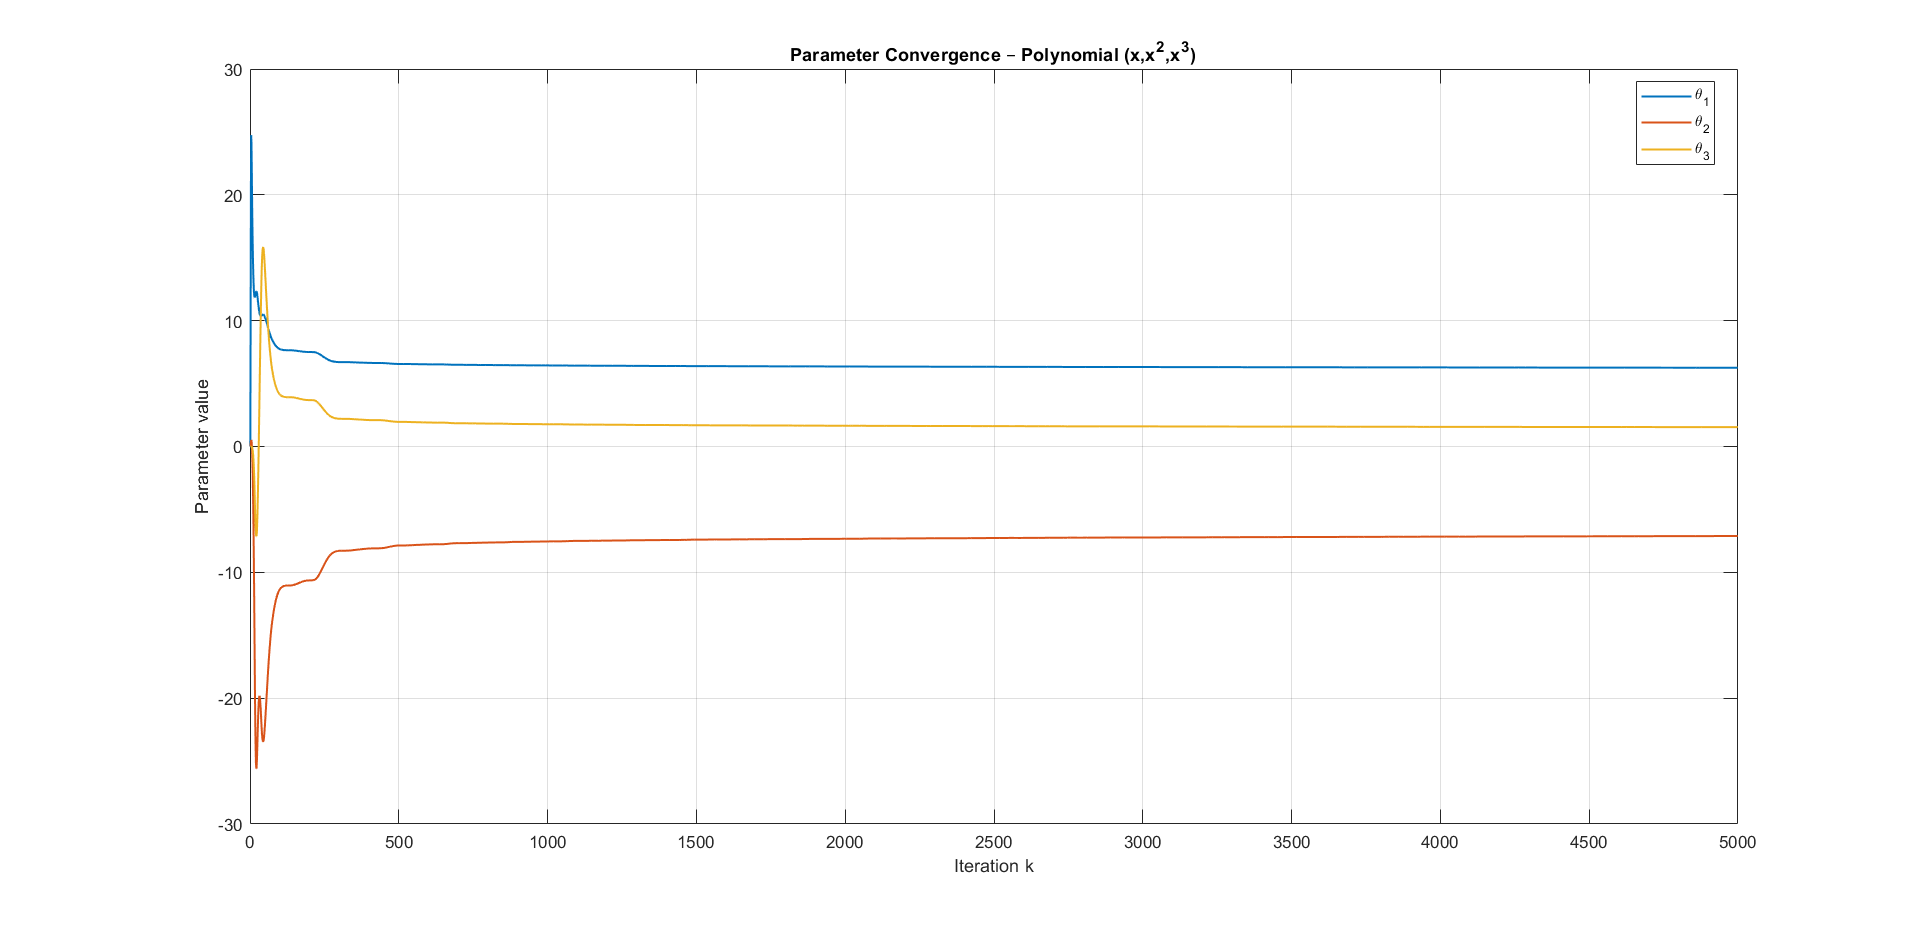
\includegraphics[width=0.96\textwidth]{PartC_fig_C.png}
    \caption{Σύγκλιση παραμέτρων για Πολυωνυμική βάση \((x, x^2, x^3)\)}
\end{figure}

\begin{figure}[H]
    \centering
    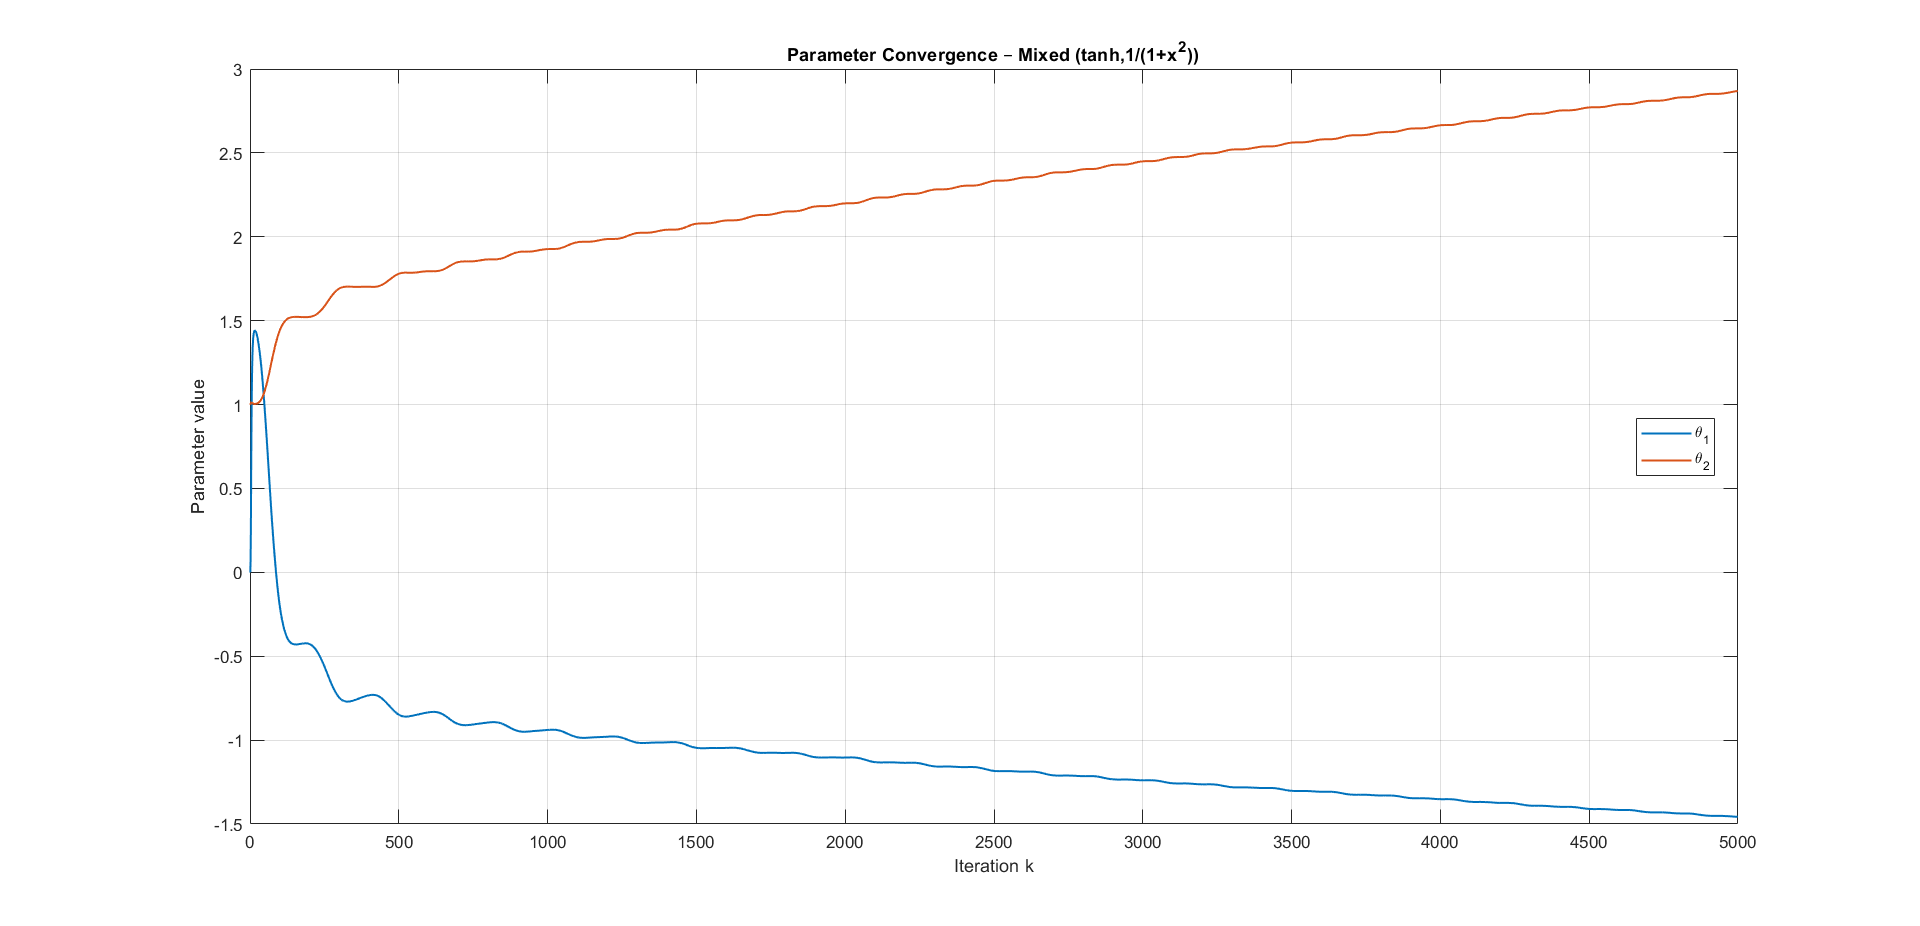
\includegraphics[width=0.96\textwidth]{PartC_fig_B.png}
    \caption{Σύγκλιση παραμέτρων για Μεικτή βάση \((\tanh(x), 1/(1+x^2))\)}
\end{figure}

\begin{figure}[H]
    \centering
    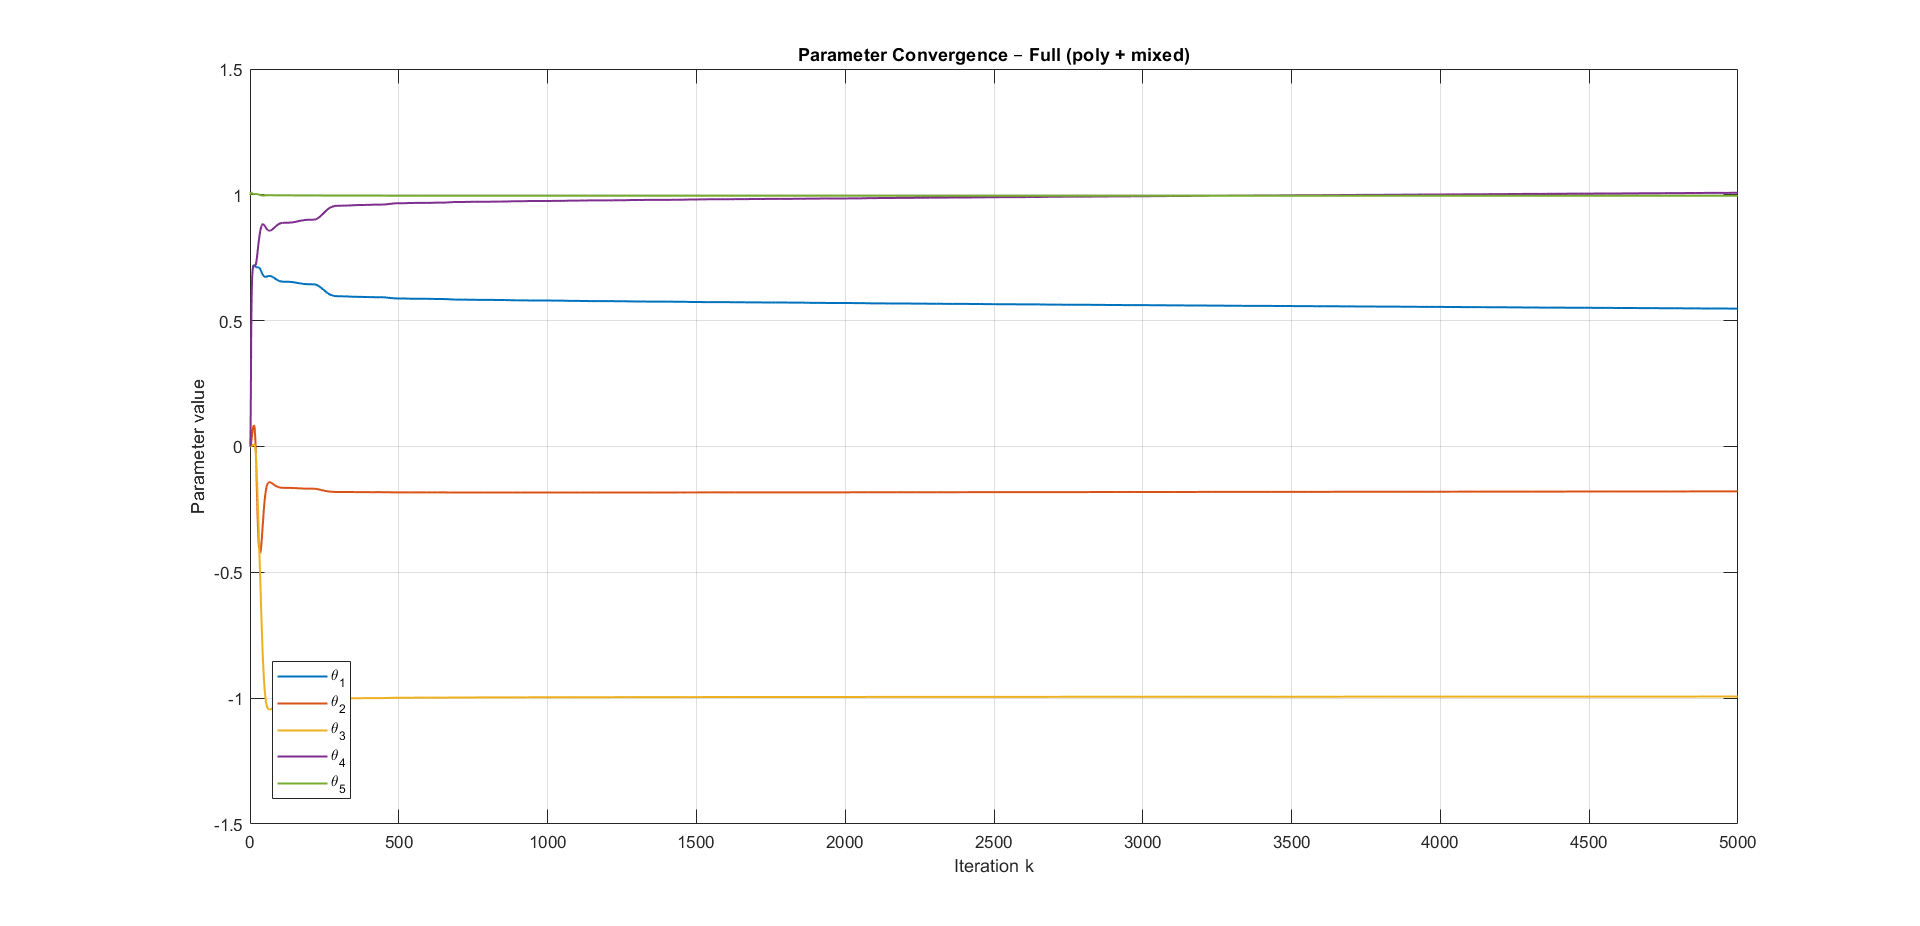
\includegraphics[width=0.96\textwidth]{PartC_fig.png}
    \caption{Σύγκλιση παραμέτρων για πλήρες μοντέλο (Πολυωνυμική + Μη γραμμική βάση)}
\end{figure}

\vspace{0.3cm}

\paragraph{Αριθμητικά Αποτελέσματα:}

\hspace{-0.25cm}Τα τελικά σφάλματα \en (MSE\gr) για κάθε υποψήφια δομή έχουν ως εξής:
\en 
\begin{table}[H]
\centering
\begin{tabular}{|l|c|}
\hline
\textbf{\gr Δομή Μοντέλου \en} & \textbf{MSE \gr στο \en Test Set\en} \\
\hline
Polynomial \((x, x^2, x^3)\) & \(5.0589 \times 10^{-5}\) \\
Mixed \((\tanh(x), \frac{1}{1+x^2})\) & \(2.9554 \times 10^{-2}\) \\
Full (Poly + Mixed) & \(\mathbf{9.1493 \times 10^{-9}}\) \\
\hline
\end{tabular}
\caption{\gr Συγκριτική απόδοση διαφορετικών δομών ως προς το μέσο τετραγωνικό σφάλμα.\en}
\end{table}
\gr

\paragraph{Παρατηρήσεις:}

\hspace{-0.25cm}Η ανάλυση των αποτελεσμάτων δείχνει ότι η πλήρης βάση, η οποία περιλαμβάνει τόσο πολυωνυμικά όσο και μη-γραμμικά χαρακτηριστικά, παρουσιάζει την καλύτερη απόδοση, με πολύ χαμηλό \en MSE\gr. Η πολυωνυμική δομή ακολουθεί με επαρκή ακρίβεια, ενώ η μεικτή μη-γραμμική δομή, παρότι περιέχει τα σωστά στοιχεία της δυναμικής, αποτυγχάνει να αναπαράγει ακριβώς την πραγματική συνάρτηση λόγω ανεπαρκούς εκφραστικότητας ως αυτόνομη. Επιπλέον, από τα γραφήματα παρατηρείται σταθερή και γρήγορη σύγκλιση των παραμέτρων για τις πιο εύρωστες δομές, ενώ στο μεικτό μοντέλο χωρίς τα πολυωνυμικά στοιχεία η σύγκλιση είναι αργή και ασταθής.

\vspace{0.3cm}

\hspace{-0.6cm} Ο αντίστοιχος κώδικας \en MATLAB \gr βρίσκεται στο αρχείο \en Part2\_a.m\gr.

\vspace{0.3cm}

\section{Θέμα 2 (β): Τελική Επιλογή Μοντέλου και Αξιολόγηση Γενίκευσης}

\subsection{Εισαγωγή στο ζητούμενο}

Το δεύτερο σκέλος του Θέματος 2 επικεντρώνεται στην τελική επιλογή μοντέλου για την προσέγγιση της άγνωστης δυναμικής $f(x,u,\theta)$ με στόχο την ελαχιστοποίηση του σφάλματος και την αξιολόγηση της γενικευσιμότητας του μοντέλου. Ειδικότερα, ζητείται:

\begin{itemize}
    \item Να επιλεγεί η δομή που επιτυγχάνει την ελαχιστοποίηση του συνολικού σφάλματος προσαρμογής:
    \[
    J(\hat{\theta}) = \int_0^t e^2(\tau) \, d\tau,
    \]
    με $e(t) = \dot{x}(t) - \hat{f}(x(t), u(t), \hat{\theta})$.
    
    \item Να ληφθεί υπόψη και η πολυπλοκότητα του υποδείγματος, μέσω του πλήθους παραμέτρων της $\hat{\theta}$ και της φύσης των συναρτήσεων βάσης $\phi(x)$.

    \item Να αξιολογηθεί η σταθερότητα και η ικανότητα γενίκευσης του τελικού μοντέλου, εφαρμόζοντάς το σε διαφορετικά σύνολα δεδομένων από αυτά που χρησιμοποιήθηκαν στην αρχική εκπαίδευση (π.χ. νέο σήμα εισόδου $u(t)$).

    \item Τέλος, να σχολιαστούν τα αποτελέσματα σε σχέση με τις επιλογές που έγιναν στο ερώτημα (α), τόσο ως προς την επιτευχθείσα ακρίβεια όσο και ως προς την αποδοτικότητα της επιλεγμένης δομής.
\end{itemize}

\hspace{-0.6cm}Η εργασία αυτή συνιστά ένα σημαντικό βήμα στη διαδικασία μοντελοποίησης, καθώς επιχειρεί να απαντήσει στο ερώτημα: 

\vspace{0.15cm}

\hspace{-0.6cm}Ποιο από τα υποδείγματα που εκπαιδεύτηκαν στο προηγούμενο στάδιο είναι τελικά το πιο κατάλληλο για να χρησιμοποιηθεί ως γενικευμένο μοντέλο, ικανό να αναπαράγει με συνέπεια τη συμπεριφορά του συστήματος και πέραν του αρχικού συνόλου εκπαίδευσης;

\vspace{0.15cm}

\hspace{-0.6cm}Και σε αυτό το ερώτημα καλούμαι να απαντήσω.

\newpage
\subsection{Θεωρητική Ανάλυση και Βασική Προσέγγιση του Προβλήματος}

Η επίλυση του Θέματος 2(β) βασίζεται στην εφαρμογή των αποτελεσμάτων του Θέματος 2(α), με στόχο την επιλογή του καταλληλότερου μοντέλου και την αξιολόγηση της σταθερότητας και γενικευσιμότητάς του. Το πρόβλημα χωρίζεται θεωρητικά σε τρία βασικά στάδια που θα αναδείξω και παρακάτω.

\hspace{-0.6cm}Η επιλογή του τελικού μοντέλου πραγματοποιείται μεταξύ των υποψηφίων δομών που εξετάστηκαν στο Θέμα 2(α), αξιοποιώντας τα αποτελέσματα της διαδικασίας εκπαίδευσης και διαχωρισμού δεδομένων.


\vspace{0.3cm}
\paragraph{Κριτήρια Επιλογής Μοντέλου – \en AIC/BIC\gr:}

\hspace{-0.25cm}Η επιλογή του βέλτιστου μοντέλου γίνεται με χρήση των στατιστικών δεικτών \en Akaike Information Criterion (AIC) \gr και \en Bayesian Information Criterion (BIC)\gr, οι οποίοι συνδυάζουν την ακρίβεια πρόβλεψης και την πολυπλοκότητα του μοντέλου:
\en
\[
\text{AIC} = N \cdot \log(\text{MSE}) + 2k, \quad
\text{BIC} = N \cdot \log(\text{MSE}) + k \cdot \log(N),
\]
\gr
όπου $N$ το πλήθος σημείων ελέγχου \en (test set)\gr, $k$ ο αριθμός παραμέτρων του μοντέλου, και $\text{\en MSE \gr}$ το μέσο τετραγωνικό σφάλμα πρόβλεψης. Το μοντέλο με την ελάχιστη τιμή \en AIC/BIC \gr επιλέγεται ως το τελικό υπόδειγμα.

\vspace{0.3cm}
\paragraph{Σταθερότητα και Απόκριση Τελικού Μοντέλου:}

\hspace{-0.25cm}Αφού επιλεγεί η τελική δομή και το διάνυσμα παραμέτρων $\hat{\theta}$, ακολουθεί δυναμική αξιολόγηση του μοντέλου υπό νέα δεδομένα. Χρησιμοποιείται νέα είσοδος $u_2(t)$, ώστε να παραχθεί η έξοδος του μοντέλου:
\en
\[
x_{\text{mod}}(k+1) = x_{\text{mod}}(k) + T_s \cdot \big( \hat{f}(x_{\text{mod}}(k), u_2(k)) \big),
\]
\gr
όπου $\hat{f}(x,u) = \phi(x)^\top \hat{\theta} + u$ είναι η προσέγγιση της δυναμικής από το εκπαιδευμένο υπόδειγμα.

\hspace{-0.6cm}Παράλληλα υπολογίζεται η αληθινή έξοδος $x_{\text{\en true\gr}}(t)$ από τη γνωστή συνάρτηση $f(x,u,\theta_{\text{\en true\gr}})$ και η διαφορά τους $e(t) = x_{\text{\en true\gr}}(t) - x_{\text{\en mod\gr}}(t)$.

\vspace{0.3cm}

\paragraph{Αξιολόγηση απόδοσης μέσω ολοκληρωμένου σφάλματος:}

\hspace{-0.25cm}Για την ποσοτική αποτίμηση της ποιότητας παρακολούθησης του συστήματος από το μοντέλο, χρησιμοποιείται το ολοκληρωμένο τετραγωνικό σφάλμα:

\[
\text{\en ISE\gr} = \int_0^T e^2(t) dt \approx \sum_{k=1}^N e_k^2 \cdot T_s = \texttt{\en trapz\gr}(t, e.^2),
\]

\hspace{-0.6cm}όπου $e_k = x_{\text{\en true\gr}}(k) - x_{\text{\en mod\gr}}(k)$ είναι η στιγμιαία απόκλιση.

\vspace{0.3cm}
\paragraph{Στόχος και Κριτήρια Επιτυχίας}

\hspace{-0.25cm}Η τελική προσέγγιση θεωρείται επιτυχής εφόσον:
\begin{itemize}
    \item Η επιλεγείσα δομή παρουσιάζει μικρότερη τιμή \en AIC/BIC \gr συγκριτικά με τις εναλλακτικές.
    \item Το ολοκληρωμένο σφάλμα \en ISE \gr είναι χαμηλό.
    \item Η έξοδος του τελικού μοντέλου παραμένει φραγμένη: $\max |x_{\text{\en mod \gr}}(t)| < \infty$.
    \item Η συμπεριφορά του μοντέλου είναι σταθερή και συγκλίνει προς τη δυναμική του συστήματος για διαφορετικές διεγέρσεις εισόδου.
\end{itemize}

\hspace{-0.6cm}Η παραπάνω θεωρητική ανάλυση ενσωματώνει τόσο στατιστικά εργαλεία μοντελοποίησης όσο και κριτήρια ευστάθειας και γενίκευσης, διαμορφώνοντας μία πλήρη προσέγγιση επιλογής και τελικής επικύρωσης μη-γραμμικών υποδειγμάτων.

\hspace{-0.6cm}Με αυτόν τον τρόπο ικανοποιείται πλήρως ο στόχος του ερωτήματος, δηλαδή η εύρεση τελικού μοντέλου που ελαχιστοποιεί το συνολικό σφάλμα μοντελοποίησης και επιδεικνύει σταθερή και γενικεύσιμη συμπεριφορά υπό νέα δεδομένα εισόδου.

\subsection{Αποτελέσματα για Οπτικοποίηση και Συμπεράσματα}

Η συνολική διαδικασία επιλογής και επικύρωσης μοντέλου οδήγησε στην επιλογή της πλήρους δομής \en full (poly and mixed)\gr, βάσει του κριτηρίου \en AIC\gr, όπως αποτυπώνεται στον ακόλουθο συγκεντρωτικό πίνακα:

\vspace{0.2cm}
\begin{center}
\begin{tabular}{|c|c|c|c|}
\hline
\textbf{Δομή} & \textbf{\en Test MSE} & \textbf{\en AIC} & \textbf{\en BIC} \\
\hline
\en poly & $5.248 \cdot 10^{-5}$ & $-49269.21$ & $-49249.66$ \\
\en mixed & $2.943 \cdot 10^{-2}$ & $-17625.31$ & $-17612.28$ \\
\en full & $9.135 \cdot 10^{-9}$ & $\mathbf{-92545.77}$ & $\mathbf{-92513.18}$ \\
\hline
\end{tabular}
\gr
\end{center}


\vspace{0.4cm}
\hspace{-0.6cm}Η τελική δομή δοκιμάστηκε σε νέα σειρά δεδομένων εισόδου $u_2(t)$ για την αξιολόγηση της σταθερότητας και της γενικευσιμότητας. Τα αποτελέσματα παρουσιάζονται στο παρακάτω σχήμα, όπου απεικονίζονται:
\begin{itemize}
    \item Η έξοδος του συστήματος $x_{\text{\en true\gr}}(t)$ έναντι της προβλεπόμενης από το μοντέλο $x_{\text{\en mod\gr}}(t)$.
    \item Το σφάλμα παρακολούθησης $e(t) = x_{\text{\en true\gr}}(t) - x_{\text{\en mod\gr}}(t)$.
    \item Η είσοδος $u(t)$ του ελέγχου.
\end{itemize}

\vspace{0.2cm}
\begin{figure}[H]
\centering
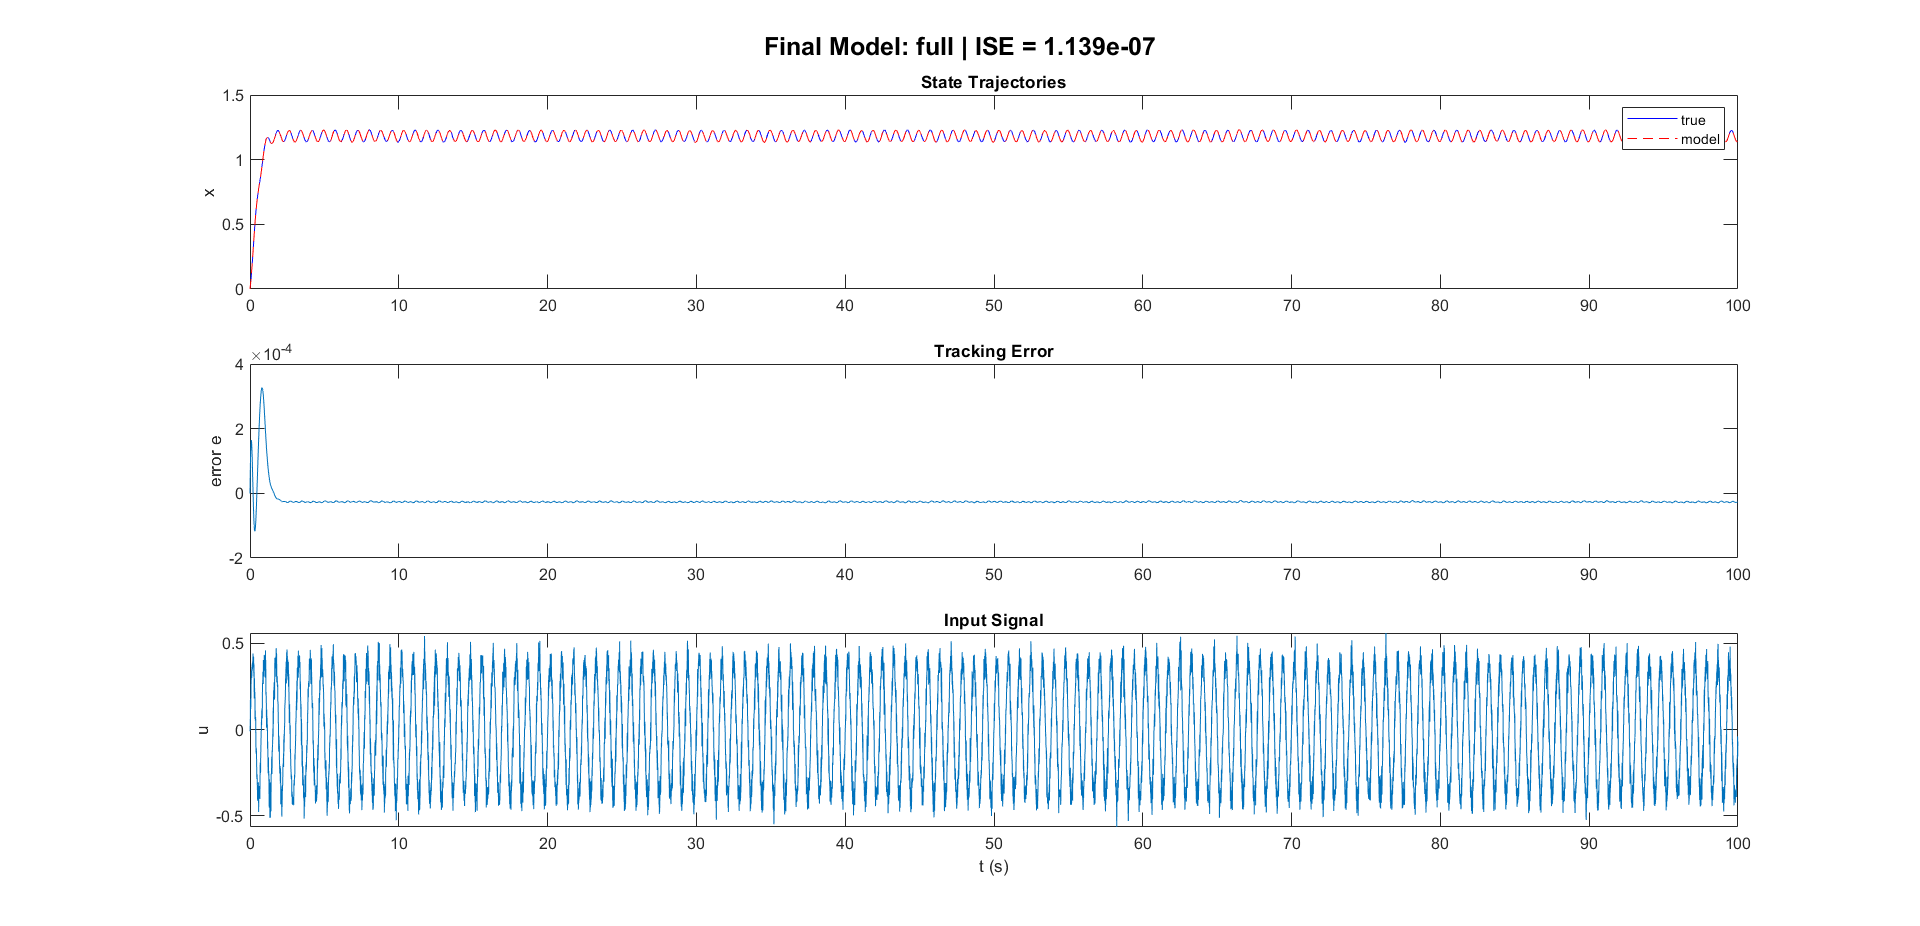
\includegraphics[width=0.96\textwidth]{PartD_fig.png}
\caption{Αξιολόγηση του τελικού μοντέλου σε νέα δεδομένα \en (full structure)\gr.}
\end{figure}

\vspace{0.4cm}
\paragraph{Παρατηρήσεις:}
\begin{itemize}
    \item Το μοντέλο \en full \gr αναπαράγει με εξαιρετική ακρίβεια την έξοδο του συστήματος, όπως φαίνεται από την επικαλυπτόμενη συμπεριφορά $x_{\text{\en mod\gr}}(t)$ και $x_{\text{\en true\gr}}(t)$.
    \item Το \textbf{ολοκληρωμένο τετραγωνικό σφάλμα \en (ISE) \gr} ήταν μόλις:
    \en
    \[
    \text{ISE} = 1.101 \cdot 10^{-7},
    \]
    \gr
    το οποίο καταδεικνύει πολύ μικρή απόκλιση για όλη τη διάρκεια $T$.
    \item Το σφάλμα παραμένει φραγμένο και μηδενίζεται ασυμπτωτικά, αποδεικνύοντας τη σταθερότητα του τελικού μοντέλου.
    \item Η έξοδος $x_{\text{\en mod\gr}}(t)$ ήταν φραγμένη με:
    \[
    \max |x_{\text{\en mod\gr}}(t)| = 1.232,
    \]
    γεγονός που επιβεβαιώνει την ευρωστία του μοντέλου σε μη εκπεδευμένα δεδομένα εισόδου.
\end{itemize}

\vspace{0.4cm}

\noindent Συμπερασματικά, το πλήρες μοντέλο επιτυγχάνει τον βέλτιστο συμβιβασμό μεταξύ πολυπλοκότητας και ακρίβειας πρόβλεψης, παρέχοντας εξαιρετική γενίκευση και σταθερή απόκριση σε άγνωστα σήματα εισόδου. Αποτελεί επομένως την καταλληλότερη επιλογή για αναπαράσταση της δυναμικής $f(x,u,\theta)$ του συστήματος.

\vspace{0.3cm}

\hspace{-0.6cm} Ο αντίστοιχος κώδικας \en MATLAB \gr βρίσκεται στο αρχείο \en Part2\_b.m\gr.

\bibliographystyle{plain}
\begin{thebibliography}{1}
    \bibitem{lnmpikas}
    \en https://elearning.auth.gr/course/view.php?id=16318
    \bibitem{second}
    \en https://bpb-us-w2.wpmucdn.com/blog.nus.edu.sg/dist/f/14858/files/2021/07/bookchapter-LyapunovDesign.pdf
    \bibitem{third}
    \en https://en.wikipedia.org/wiki/Euler\_method
\end{thebibliography}

\end{document}